\documentclass[10pt]{jarticle}
\usepackage[dvipdfmx]{graphicx}
\usepackage[dvipdfmx]{color}
\usepackage{here}
\usepackage[top=30truemm, bottom=20truemm, left=30truemm, right=30truemm]{geometry}



\title{原子核の変形と中性子ドリップラインに対するクーロン相互作用の効果}
\author{萩原健太}
\date{2023年1月21日}
\begin{document}

\begin{center}
  {\Large
    原子核の変形と中性子ドリップラインに対する\\
    クーロン相互作用の効果
  }
\end{center}

\begin{flushright}
  \vskip\baselineskip201910867 萩原健太\\
  指導教員:中務孝
\end{flushright}

\section*{概要}
陽子と中性子が集まった量子多体系である原子核を扱うエネルギー密度汎関数理論が発展してきた。
この理論を用いることで、比較的小さな質量数の原子核から超重核と呼ばれる質量数の大きな原子核、さらには中性子星などのマクロな核物質までを対象に、系統的な数値計算を実行することが出来る。
本研究では原子核の変形と対相関を自己無撞着に決定することのできる計算プログラムであるHFBTHOを用い、陽子数$Z=2-120$の、束縛する全ての偶偶核を対象に数値計算を実行した。
図1に原子核の変形度を示す。
ただし原子核の形に関しては、パリティ対称性と軸対称性を破らないように制限している。
陽子・中性子の化学ポテンシャルが負であることを束縛条件として原子核の存在限界 (ドリップライン)を決定し、クーロン相互作用が偶偶核の変形度および中性子ドリップラインに与える影響について評価した。\\
計算の結果からクーロン相互作用により、原子核全体で変形度が大きくなる傾向にあること、そして興味深いことに、中性子ドリップラインが拡大することが判明した。
斥力の効果からエネルギー的には不安定になることが直感的に予想されるが、結果的に中性子ドリップライン側の束縛状態にある原子核を増やすような計算結果を得た。\\
本研究で発見された斥力のクーロン相互作用が一部の原子核を安定化させる現象は、我々の知る限り過去に指摘されたことがなく、この原因を詳しく考察することは重要である。
クーロン相互作用によって、原子核の半径や一粒子エネルギー、変形度など様々な物理量がどのように変化するのかを解析し、原子核の量子性が果たす重要な役割が解明された。
\begin{figure}[H]
  \centering
  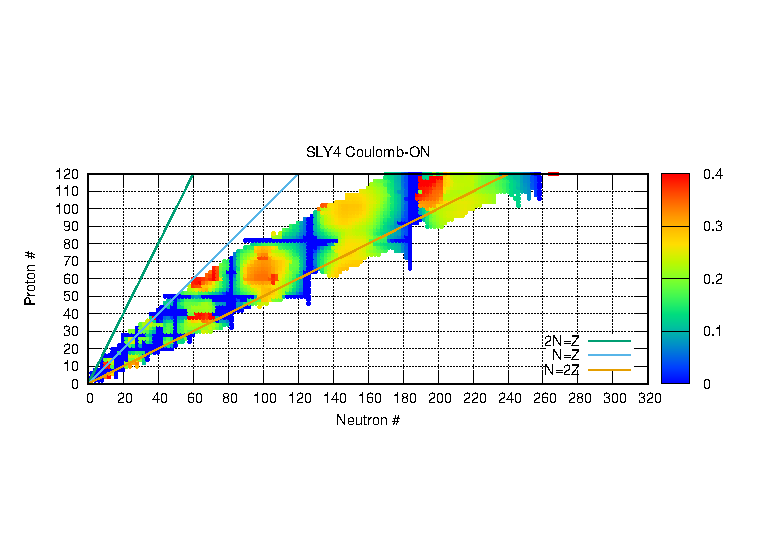
\includegraphics{../SLY4_ON.eps}
  \setlength\floatsep{0pt}
  \setlength\intextsep{0pt} 
  \setlength\textfloatsep{0pt}
  \caption{クーロン相互作用を含んだ計算で束縛状態として求まった原子核の四重極変形度の大きさ}
  \label{fig:SLY4_deformation}
\end{figure}

\end{document}